\documentclass{article}
\usepackage[margin=1in]{geometry}
\usepackage{amsmath,amsthm,amssymb}
\usepackage{bbm,enumerate,mathtools}
\usepackage{tikz,pgfplots}
\usepackage{chessboard}
\usepackage[hidelinks]{hyperref}
\usepackage{multicol} % Problem 35

\newenvironment{question}{\begin{trivlist}\item[\textbf{Question.}]}{\end{trivlist}}
\newenvironment{note}{\begin{trivlist}\item[\textbf{Note.}]}{\end{trivlist}}
\newenvironment{references}{\begin{trivlist}\item[\textbf{References.}]}{\end{trivlist}}
\newenvironment{related}{\begin{trivlist}\item[\textbf{Related.}]\end{trivlist}\begin{enumerate}}{\end{enumerate}}

\usetikzlibrary{patterns}

\begin{document}
\rating{2}{4}

It is known that trapezoids consisting of $1$, $3$, and $5$ equilateral
triangles in a line can tile an equilateral triangle.
\begin{figure}[ht!]
  \centering
  \hspace{0.5cm}
  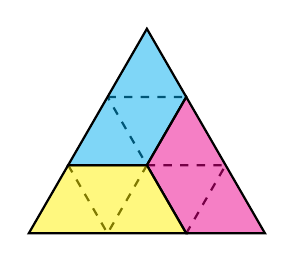
\begin{tikzpicture}
    \draw[thick, dashed]
      (1,0)--(2,0)--(1.5, {-sqrt(3)/2})
      (0,0)--(0.5, {-sqrt(3)/2})--(1,0)--(0.5,{sqrt(3)/2})
      (0.5,{sqrt(3)/2})--(1.5,{sqrt(3)/2});
    \draw[thick, fill=cyan, fill opacity=0.5] (0,0)--(1,{sqrt(3)})--(1.5,{sqrt(3)/2})--(1,0)--cycle;
    \draw[thick, fill=magenta, fill opacity=0.5] (1.5,{sqrt(3)/2})--(2.5,{-sqrt(3)/2})--(1.5,{-sqrt(3)/2})--(1,0)--cycle;
    \draw[thick, fill=yellow, fill opacity=0.5] (-0.5,{-sqrt(3)/2})--(0,0)--(1,0)--(1.5,{-sqrt(3)/2})--cycle;
  \end{tikzpicture}
  \\~\\
  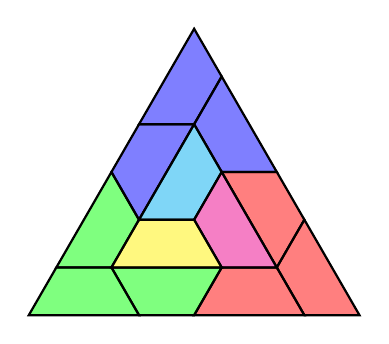
\begin{tikzpicture}[scale=0.7]
    \draw[thick, fill=green, fill opacity=0.5] (0,0)--(1,{sqrt(3)})--(1.5,{sqrt(3)/2})--(1,0)--cycle;
    \draw[thick, fill=blue, fill opacity=0.5] (1,{sqrt(3)})--(1.5,{sqrt(3)/2})--(2.5, {3/2*sqrt(3)})--(1.5, {3/2*sqrt(3)})--cycle;
    \draw[thick, fill=blue, fill opacity=0.5] (1.5,{3/2*sqrt(3)})--(2.5,{5/2*sqrt(3)})--(3,{2*sqrt(3)})--(2.5,{3/2*sqrt(3)})--cycle;
    \draw[thick, fill=blue, fill opacity=0.5] (3,{2*sqrt(3)})--(4,{sqrt(3)})--(3,{sqrt(3)})--(2.5,{3/2*sqrt(3)})--cycle;
    \draw[thick, fill=red, fill opacity=0.5] (4,0)--(3,{sqrt(3)})--(4,{sqrt(3)})--(4.5,{sqrt(3)/2})--cycle;
    \draw[thick, fill=red, fill opacity=0.5] (4,0)--(4.5,{sqrt(3)/2})--(5.5,{-sqrt(3)/2})--(4.5,{-sqrt(3)/2})--cycle;
    \draw[thick, fill=red , fill opacity=0.5] (4.5,{-sqrt(3)/2})--(4,0)--(3,0)--(2.5,{-sqrt(3)/2})--cycle;
    \draw[thick, fill=green, fill opacity=0.5] (2.5,{-sqrt(3)/2})--(3,0)--(1,0)--(1.5,{-sqrt(3)/2})--cycle;
    \draw[thick, fill=green, fill opacity=0.5] (-0.5,{-sqrt(3)/2})--(0,0)--(1,0)--(1.5,{-sqrt(3)/2})--cycle;

    \draw[thick, fill=cyan, fill opacity=0.5] (1.5,{sqrt(3)/2})--(2.5,{3/2*sqrt(3)})--(3,{sqrt(3)})--(2.5,{sqrt(3)/2})--cycle;
    \draw[thick, fill=magenta, fill opacity=0.5] (3,{sqrt(3)})--(4,0)--(3,0)--(2.5,{sqrt(3)/2})--cycle;
    \draw[thick, fill=yellow, fill opacity=0.5] (1,0)--(1.5,{sqrt(3)/2})--(2.5,{sqrt(3)/2})--(3,0)--cycle;
    % \node at (2.5,-1.3) {(primitive)};
  \end{tikzpicture}
  \hspace{0.5cm}
  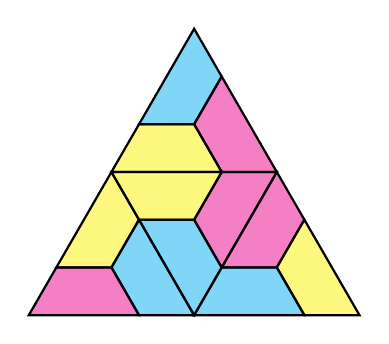
\begin{tikzpicture}[scale=0.7]
    \draw[thick, fill=yellow, fill opacity=0.5] (0,0)--(1,{sqrt(3)})--(1.5,{sqrt(3)/2})--(1,0)--cycle;
    \draw[thick, fill=cyan, fill opacity=0.5] (1.5,{sqrt(3)/2})--(2.5,{-sqrt(3)/2})--(1.5,{-sqrt(3)/2})--(1,0)--cycle;
    \draw[thick, fill=magenta, fill opacity=0.5] (-0.5,{-sqrt(3)/2})--(0,0)--(1,0)--(1.5,{-sqrt(3)/2})--cycle;

    % Lower right
    \draw[thick, fill=magenta, fill opacity=0.5] (3,0)--(4,{sqrt(3)})--(4.5,{sqrt(3)/2})--(4,0)--cycle;
    \draw[thick, fill=yellow, fill opacity=0.5] (4.5,{sqrt(3)/2})--(5.5,{-sqrt(3)/2})--(4.5,{-sqrt(3)/2})--(4,0)--cycle;
    \draw[thick, fill=cyan, fill opacity=0.5] (2.5,{-sqrt(3)/2})--(3,0)--(4,0)--(4.5,{-sqrt(3)/2})--cycle;

    % Upper
    \draw[thick, fill=cyan, fill opacity=0.5] (1.5,{3/2*sqrt(3)})--(2.5,{5/2*sqrt(3)})--(3,{2*sqrt(3)})--(2.5,{3/2*sqrt(3)})--cycle;
    \draw[thick, fill=magenta, fill opacity=0.5] (3,{2*sqrt(3)})--(4,{sqrt(3)})--(3,{sqrt(3)})--(2.5,{3/2*sqrt(3)})--cycle;
    \draw[thick, fill=yellow, fill opacity=0.5] (1,{sqrt(3)})--(1.5,{3/2*sqrt(3)})--(2.5,{3/2*sqrt(3)})--(3,{sqrt(3)})--cycle;

    % Upside down
    \draw[thick, fill=cyan, fill opacity=0.5] (1.5,{1/2*sqrt(3)})--(2.5,{-1/2*sqrt(3)})--(3,0)--(2.5,{1/2*sqrt(3)})--cycle;
    \draw[thick, fill=magenta, fill opacity=0.5] (3,0)--(4,{sqrt(3)})--(3,{sqrt(3)})--(2.5,{1/2*sqrt(3)})--cycle;
    \draw[thick, fill=yellow, fill opacity=0.5] (1,{sqrt(3)})--(1.5,{1/2*sqrt(3)})--(2.5,{1/2*sqrt(3)})--(3,{sqrt(3)})--cycle;
  \end{tikzpicture}
  \hspace{0.5cm}
  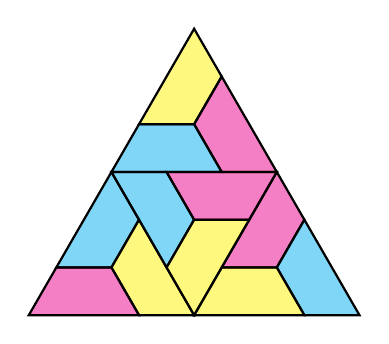
\begin{tikzpicture}[scale=0.7]
    \draw[thick, fill=cyan, fill opacity=0.5] (0,0)--(1,{sqrt(3)})--(1.5,{sqrt(3)/2})--(1,0)--cycle;
    \draw[thick, fill=yellow, fill opacity=0.5] (1.5,{sqrt(3)/2})--(2.5,{-sqrt(3)/2})--(1.5,{-sqrt(3)/2})--(1,0)--cycle;
    \draw[thick, fill=magenta, fill opacity=0.5] (-0.5,{-sqrt(3)/2})--(0,0)--(1,0)--(1.5,{-sqrt(3)/2})--cycle;

    % Lower right
    \draw[thick, fill=magenta, fill opacity=0.5] (3,0)--(4,{sqrt(3)})--(4.5,{sqrt(3)/2})--(4,0)--cycle;
    \draw[thick, fill=cyan, fill opacity=0.5] (4.5,{sqrt(3)/2})--(5.5,{-sqrt(3)/2})--(4.5,{-sqrt(3)/2})--(4,0)--cycle;
    \draw[thick, fill=yellow, fill opacity=0.5] (2.5,{-sqrt(3)/2})--(3,0)--(4,0)--(4.5,{-sqrt(3)/2})--cycle;

    % Upper
    \draw[thick, fill=yellow, fill opacity=0.5] (1.5,{3/2*sqrt(3)})--(2.5,{5/2*sqrt(3)})--(3,{2*sqrt(3)})--(2.5,{3/2*sqrt(3)})--cycle;
    \draw[thick, fill=magenta, fill opacity=0.5] (3,{2*sqrt(3)})--(4,{sqrt(3)})--(3,{sqrt(3)})--(2.5,{3/2*sqrt(3)})--cycle;
    \draw[thick, fill=cyan, fill opacity=0.5] (1,{sqrt(3)})--(1.5,{3/2*sqrt(3)})--(2.5,{3/2*sqrt(3)})--(3,{sqrt(3)})--cycle;

    % Upside down
    \draw[thick, fill=cyan, fill opacity=0.5] (1,{sqrt(3)})--(2,0)--(2.5,{1/2*sqrt(3)})--(2,{sqrt(3)})--cycle;
    \draw[thick, fill=yellow, fill opacity=0.5] (2.5,{-1/2*sqrt(3)})--(3.5,{1/2*sqrt(3)})--(2.5,{1/2*sqrt(3)})--(2,0)--cycle;
    \draw[thick, fill=magenta, fill opacity=0.5] (2,{sqrt(3)})--(2.5,{1/2*sqrt(3)})--(3.5,{1/2*sqrt(3)})--(4,{sqrt(3)})--cycle;
  \end{tikzpicture}


  \caption{
    A equilateral triangle made of $3$-trapezoids.
  }
\end{figure}
\begin{question}
  Can all $(2n-1)$-trapezoids be arranged to form an equilateral triangle?
\end{question}

\begin{related}
  \item What is the smallest triangle that can be formed this way?
  \item Is there a construction that makes such triangles given some $k$-trapezoid?
  \item How many such tilings exist for a given size trapezoid and triangle?
  \item Can other shapes be tiled (e.g. hexagon, arbitrary trapezoid)?
  \item Does this generalize to square/hexagonal tilings? Multiple dimensions?
\end{related}

\begin{note}
  If $c(n)$ counts the number of distinct minimal covering sets of $n$-ominoes,
  then $c(1) = c(2) = c(3) = 1$, $c(4) = c(5) = 2$, and $c(6) = 14$.
\end{note}

\begin{references}
  \item Problem 75
  \item \url{https://math.stackexchange.com/q/2215781/121988}
\end{references}
\end{document}
